\documentclass{article} % For LaTeX2e
% We will use NIPS submission format
\usepackage{nips13submit_e,times}
% for hyperlinks
\usepackage{hyperref}
\usepackage{placeins}
\usepackage{url}
% For figures
\usepackage{graphicx} 
% math packages
\usepackage{amsmath}
\usepackage{amsfonts}
\usepackage{amsopn}
\usepackage{ifthen}
\usepackage{natbib}
\usepackage{caption}
\usepackage{subcaption}

\usepackage{booktabs}
\newcommand{\ra}[1]{\renewcommand{\arraystretch}{#1}}

\title{Convolutional Neural Networks using separable filters}
\author{
\fontsize{8}{8}\selectfont{Petrescu Viviana}\\
\fontsize{8}{8}\selectfont{EPFL} \\
\fontsize{8}{8}\selectfont{\texttt{viviana.petrescu@epfl.ch}} \\
}

\nipsfinalcopy 

\begin{document}

\maketitle

\begin{abstract}
CNN are the state-of-the-art machine learning techniques which achieved best results on various computer vision tasks ranging from the large scale ImageNet object recognition challenge to segmentation in bio medical imaging.
This technical report presents initial results on using CNN with separable filters for speeding up the testing time.
\end{abstract}

\section{Introduction}
Although proven to be very powerful, CNN are much slower for both training and testing than their counter parts SVM or Random Forests.
In the forward pass, the computational complexity of evaluating one image of size $W\times H$ with $J$ filters of size $d_{1}\times d_{2}$ is $O(WHJd_{1}d_{2})$.
 
 Although improving the training time would be very beneficial since it would allow for more configurations to be tried and for larger networks, increasing effort has been put also into speeding up only testing time, since training can be done offline.

\section{Speeding up CNN}
By far the most common approach for speeding up CNNs is to run them on the GPU, making use of the paralelism nature of the algorithm. Alternatively or combined, FFT can be used for the convolutional operations (for  both training and testing)\cite{DBLP:journals/corr/MathieuHL13}.  For testing, a significant speedup can be obtained in hardware by using FGPAs \citep{lecun2010convolutional}. The major drawback of FGPAs is that they are harder to program for people who do not work in the field.

 In \citep{Jaderberg14b} they prove speedup of CNNs for two different schemes using separable filters, one of which is similar with our approach but uses a different optimization algorithm for obtaining the separable filters. 
  If the $2D$ filters are decomposed into a set of separable $1D$ filters of rank $K$, the complexity per image becomes
 $O(WH(J +d_{1}+d_{2}))$. Thus, we obtain a speedup if $K<< \frac{Jd_{1}d_{2}}{J +d_{1}+d_{2}}$. 

\section{Separable filters}
In our approach, the set of filters $\chi$ for one convolutional layer is approximated as
a set of separable filters, as shown in Fig\ref{fig:decomposition}.
\begin{figure}[h]
  \centering
   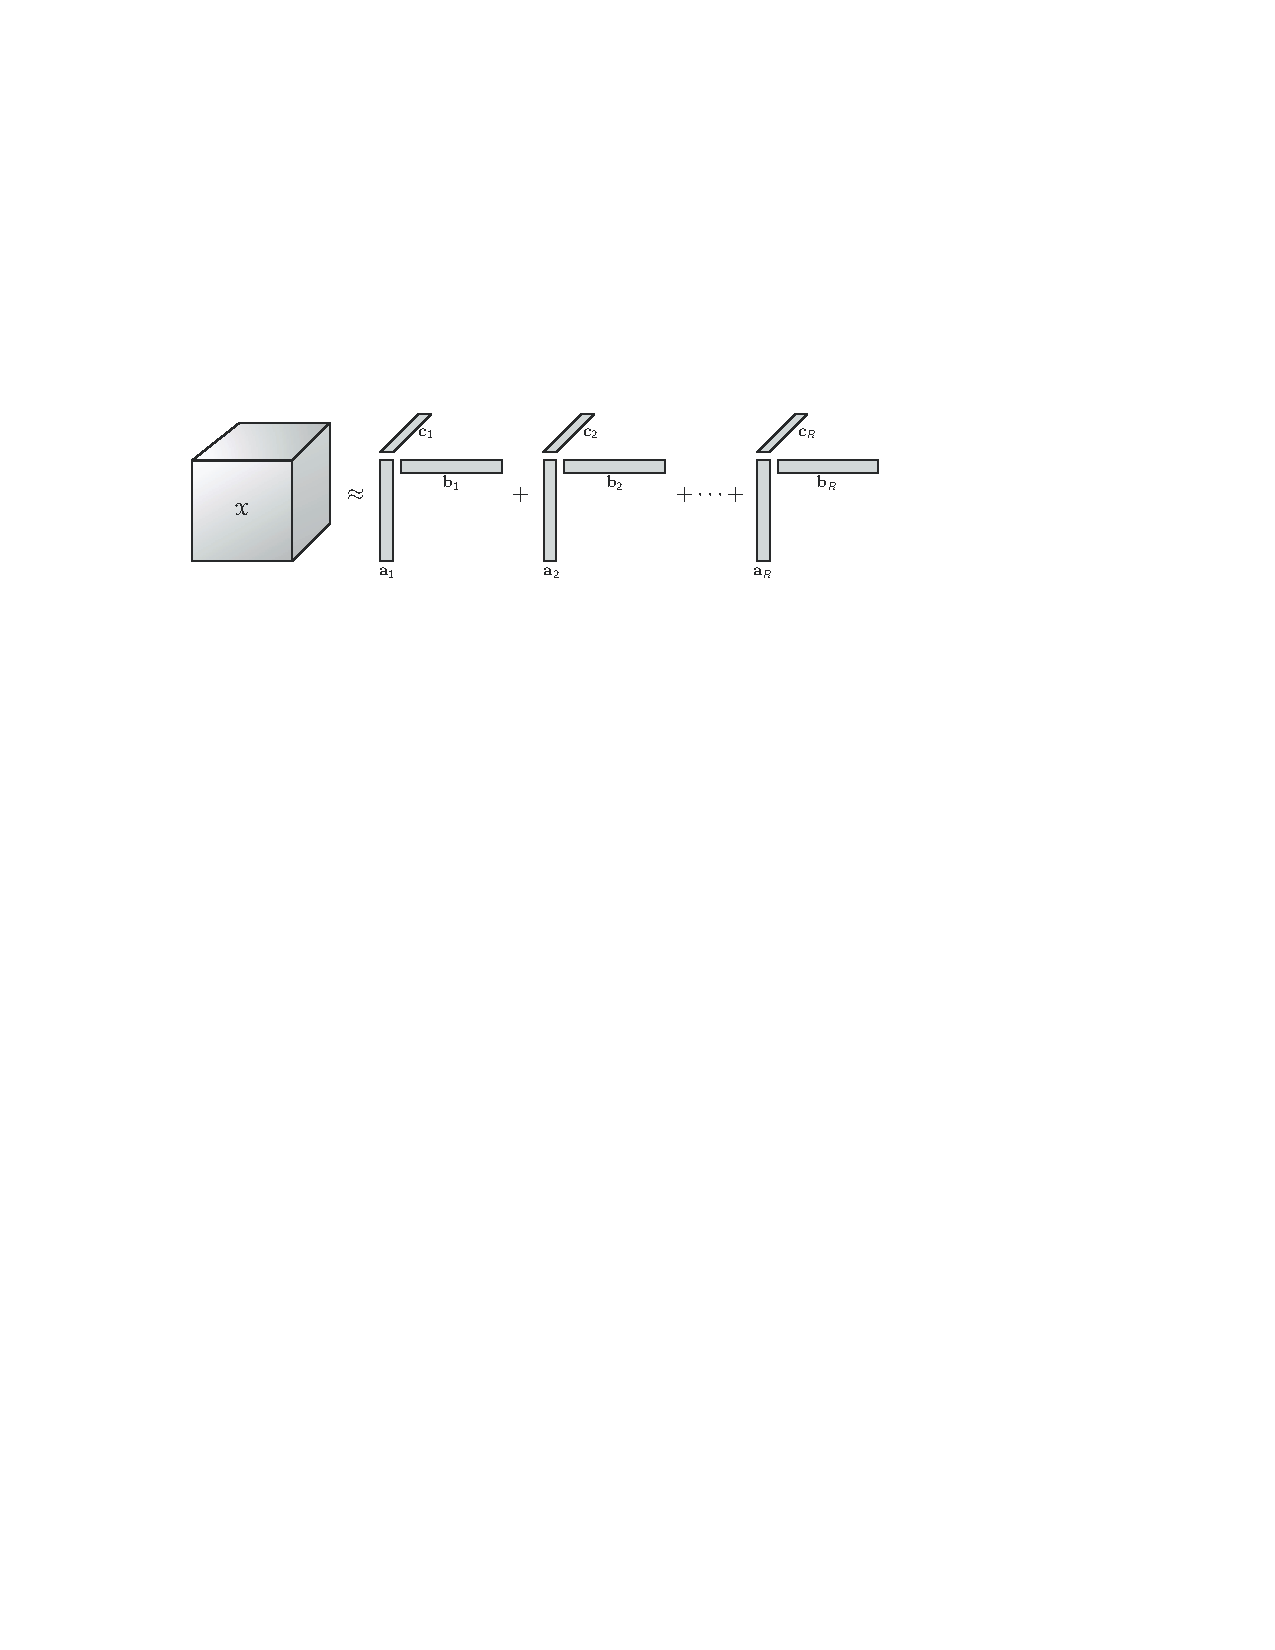
\includegraphics[width=\textwidth]{images/decomposable.pdf}
  \caption{Tensor decomposition}
  \label{fig:decomposition}
\end{figure}

We can obtain an approximation by minimizing the equation:
\begin{equation*}
\begin{aligned}
& \underset{a,b,c}{\text{minimize}}
& \| \chi - \sum_{r=1}^{r=R}{a_{r}\circ b_{r}\circ c_{r}} \|_{2}^{2} 
\end{aligned}
\end{equation*}
We optimize the above equation using a Matlab implementation of the Canonical Polyadic decomposition (a generalization of  SVD for tensors) with  non linear conjugate gradient method. The optimization framework requires as input the rank $R$, which is almost never known. When the rank used for decomposition is not the theoretical one, the decomposition is not very accurate and the algorithm needs to be run with different initialization parameter until it converges.
What is known is an upper bound on the theoretical rank $R$ for a  general tensor $3D$ tensor $\chi \in \mathbb{R}^{I\times J\times K}$, given by:
 \begin{equation*}
\begin{aligned}
& \text{rank}(\chi) \leq 
& min{\{IJ, JK, KI\}}
\end{aligned}
\end{equation*} 
Besides the theoretical rank, there is also the notion of typical rank, which is any rank
that appears with probability greater than 0, or that it is most common \cite{KoBa09}.
Some of the known typical ranks are shown in Table \ref{table:rank}.
Looking at the first row of Table \ref{table:rank}, we conclude that for a 'very tall' set of filters like the ones present in large CNNs, 
we should expect the rank to be equal with the product of the two kernel dimensions.
 \begin{table}
\centering
\begin{tabular}{@{}ll@{}}\toprule
Tensor size & Typical rank \\ \midrule
$I \times J \times K$ with $JK \leq I$ (very tall) & $JK$\\
$I \times J \times K$ with $JK - J < I < JK$ (tall) & $I$ \\
$I \times J \times K$ with $I = JK - J$ (compact) & $I, I+1$  \\ \bottomrule
\end{tabular}
\caption{Typical rank for certain tensor shapes}
\label{table:rank}
\end{table}

\section{Experiments}
We ran the experiments in Python, using the Theano library. 
We varied the rank for every convolutional layer and compared the separable version with the non separable one. We recorded the time, the change in performance and how well the separable filters approximate the $2D$ filters. We experimented on the MNIST and on the Mitocondria Striatum datasets.

\subsection{MNIST}
MNIST consists of a curated set of grayscale images (28x28) depicting handwritten digits.
The dataset is split into 60.000 training samples, 10.000 validation and 
10.000 testing samples. For this set, the approach of \cite{DBLP:journals/corr/abs-1202-2745} using CNNs is the best  model with a 0.23 error rate (23 out of 10.000 digits not recognized correctly).
We start our experience with the reference Theano model for MNIST which achieves 0.82 error rate. Its configuration is shown in Table\ref{fig:cnn1}
\subsubsection{CNN Model 1}
\begin{table}[h!]
\centering
\begin{tabular}{@{}rlll@{}}\toprule
Layer & Type & Maps and neurons& Kernel size \\ \midrule
0 & input & 1 map of 28x28 &\\
1& convolutional & 20 maps of 24x24 & 5x5\\
2 & max pooling & 20 maps of 12x12 &  \\
3 & convolutional & 50 maps of 8x8& 5x5 \\
4 & max pooling & 50 maps of 4x4&  \\ 
5 & fully conntected& 500 & \\
6 & fully conntected & 2 neurons & \\ \bottomrule
\end{tabular}
\caption{CNN Model 1 for MNIST}
\label{fig:cnn1}
\end{table}

We decompose the filter map from the first convolutional layer. From the theoretical point of view, according to Table \ref{table:rank}, we have a compact tensor $R^{20\times 5 \times 5}$ with a typical rank of 20 or 21, so we expect a very good aproximation for a rank in that range. 
Fig\ref{fig:cnn1fitness}a shows how well is the approximation with varying rank from 4 to 16 in steps of 2 on the $x$ axis and the fit on the $y$ axis (100 corresponds to perfect fit). As expected, the fit is almost perfect for high ranks and decreases afterwards.

Using separable filters, we obtain a theoretical speedup for convolutional layer 1 if $K<< \frac{Jd_{1}d_{2}}{J +d_{1}+d_{2}} = \frac{20\times 5\times 5}{20 + 5 + 5} = 16.66$. Fig\ref{fig:cnn1time}a shows the time improvements using separable filters. The blue line represents the time per layer using non separable filters. In our implementation, the separable filters give a speedup for any rank, as the red curve is below the blue one. 
We note that theoretically using non separable filters (blue line) and using separable filters with rank 16 should have given the same running time. The reason for the difference is due to implementation details and it is a language specific artifact.

\begin{figure}[h!]
  \centering
  \begin{subfigure}[b]{0.40\textwidth}
   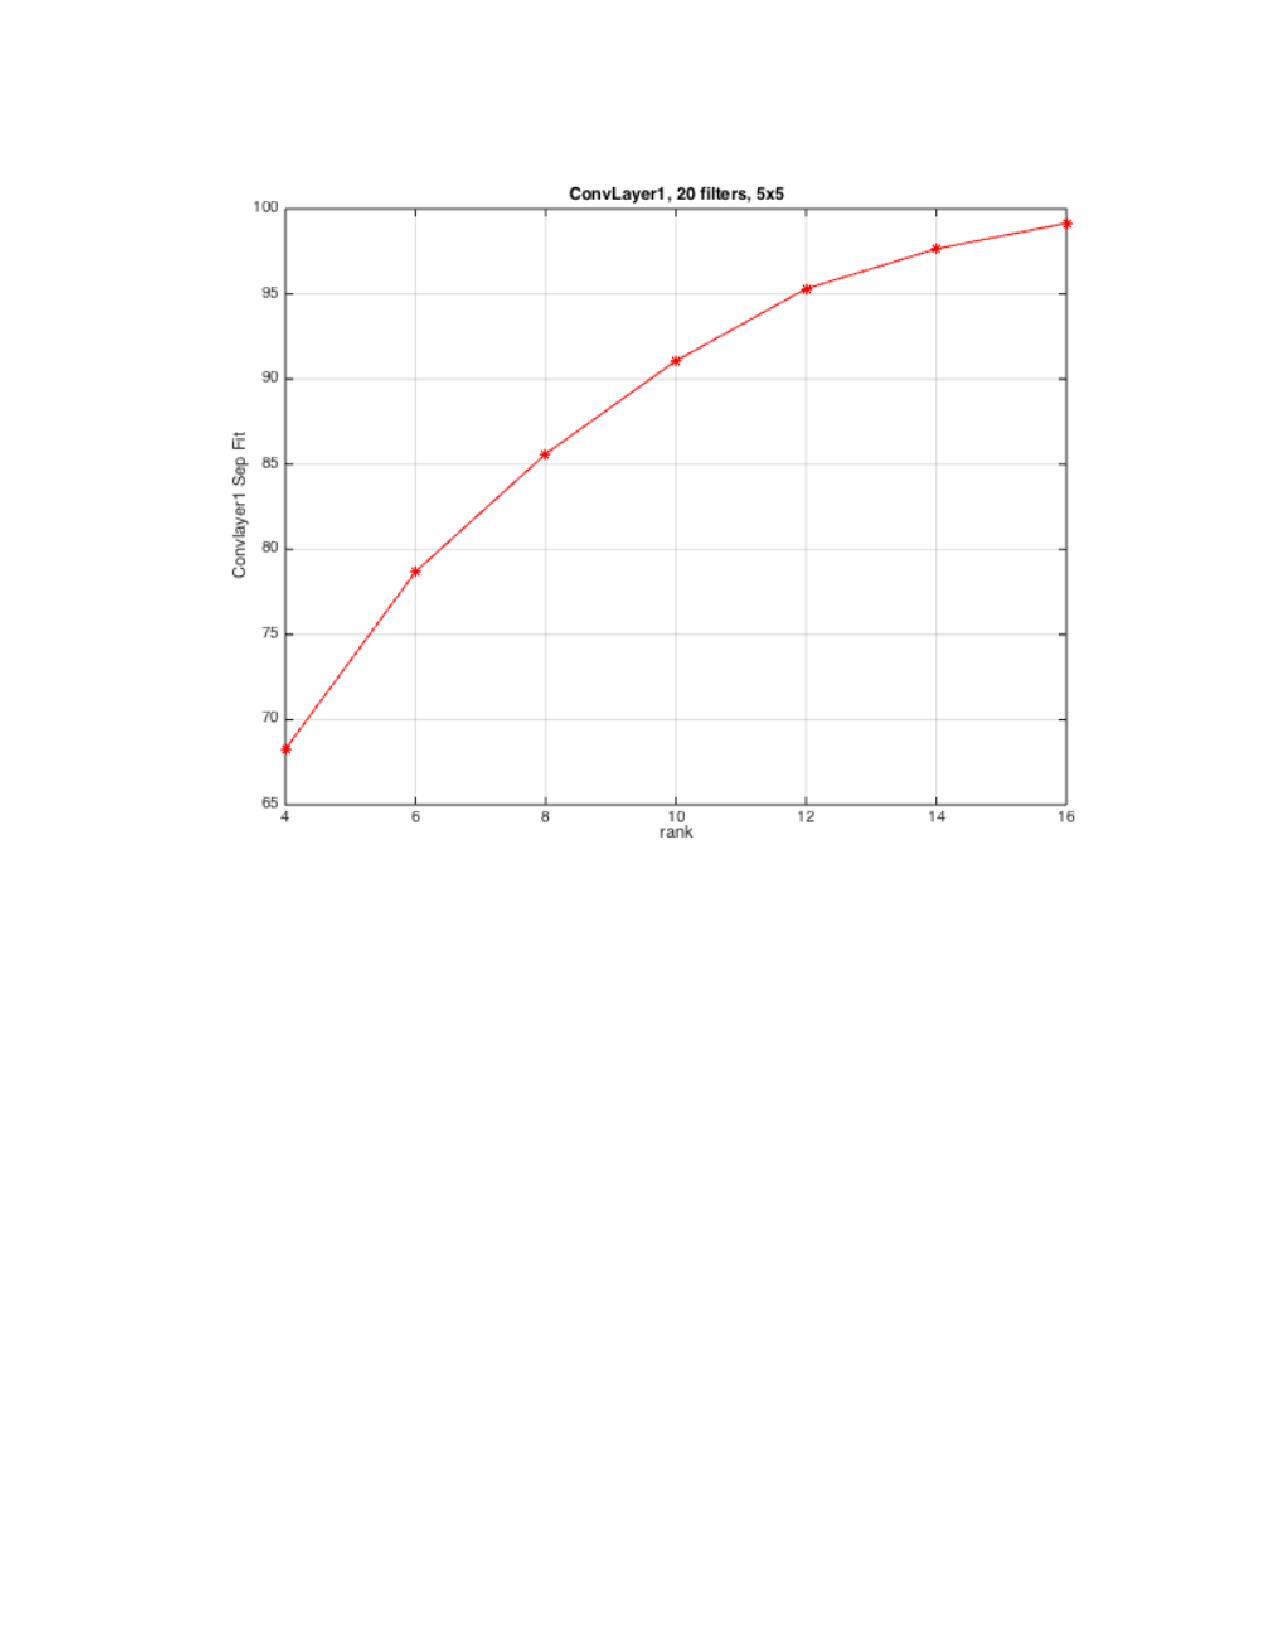
\includegraphics[width=\textwidth]{images/imagesCNN_page6.pdf}
    \caption{Convolutional layer 1}
  \end{subfigure}
  \begin{subfigure}[b]{0.40\textwidth}
    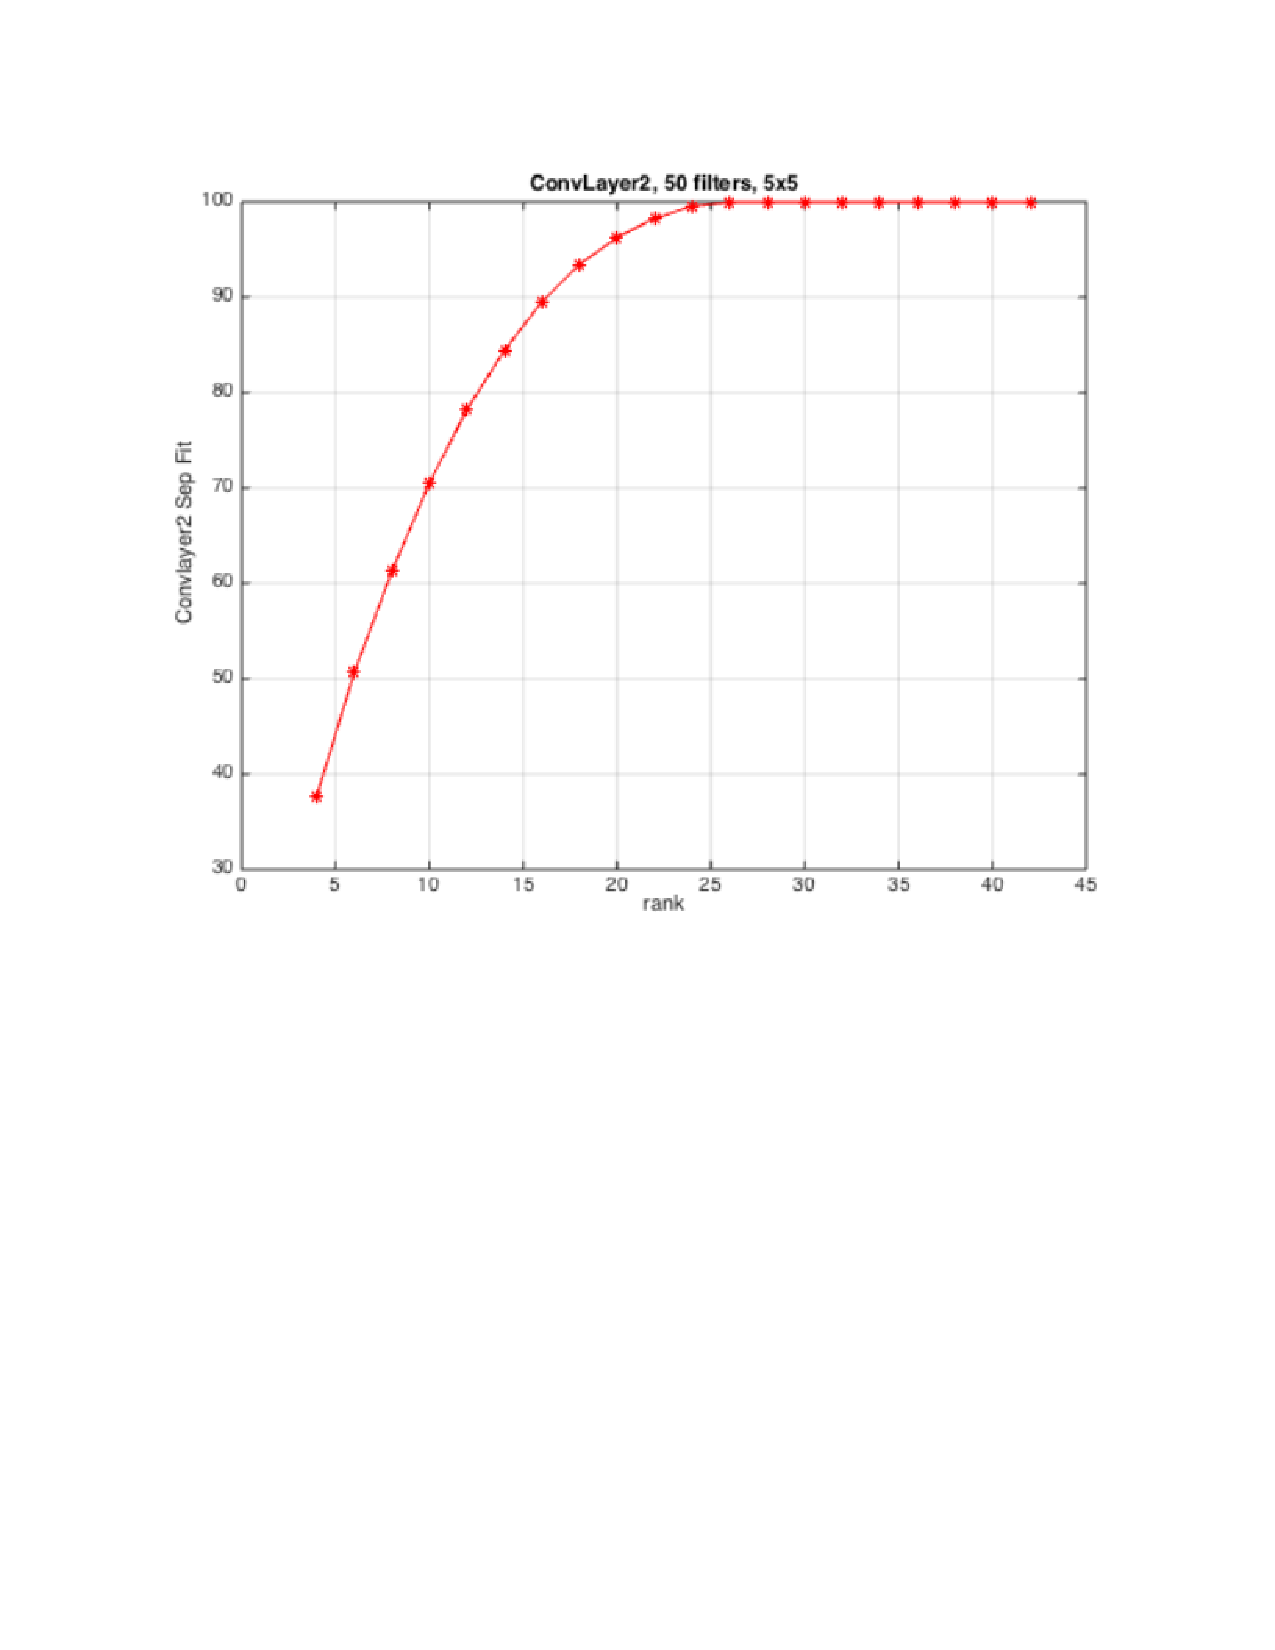
\includegraphics[width=\textwidth]{images/imagesCNN_page2.pdf}
    \caption{Convolutional layer 2}
  \end{subfigure}
  \caption{CNN Model 1 MNIST. Rank vs Fit}
  \label{fig:cnn1fitness}
\end{figure}

\begin{figure}[h!]
  \centering
  \begin{subfigure}[b]{0.40\textwidth}
   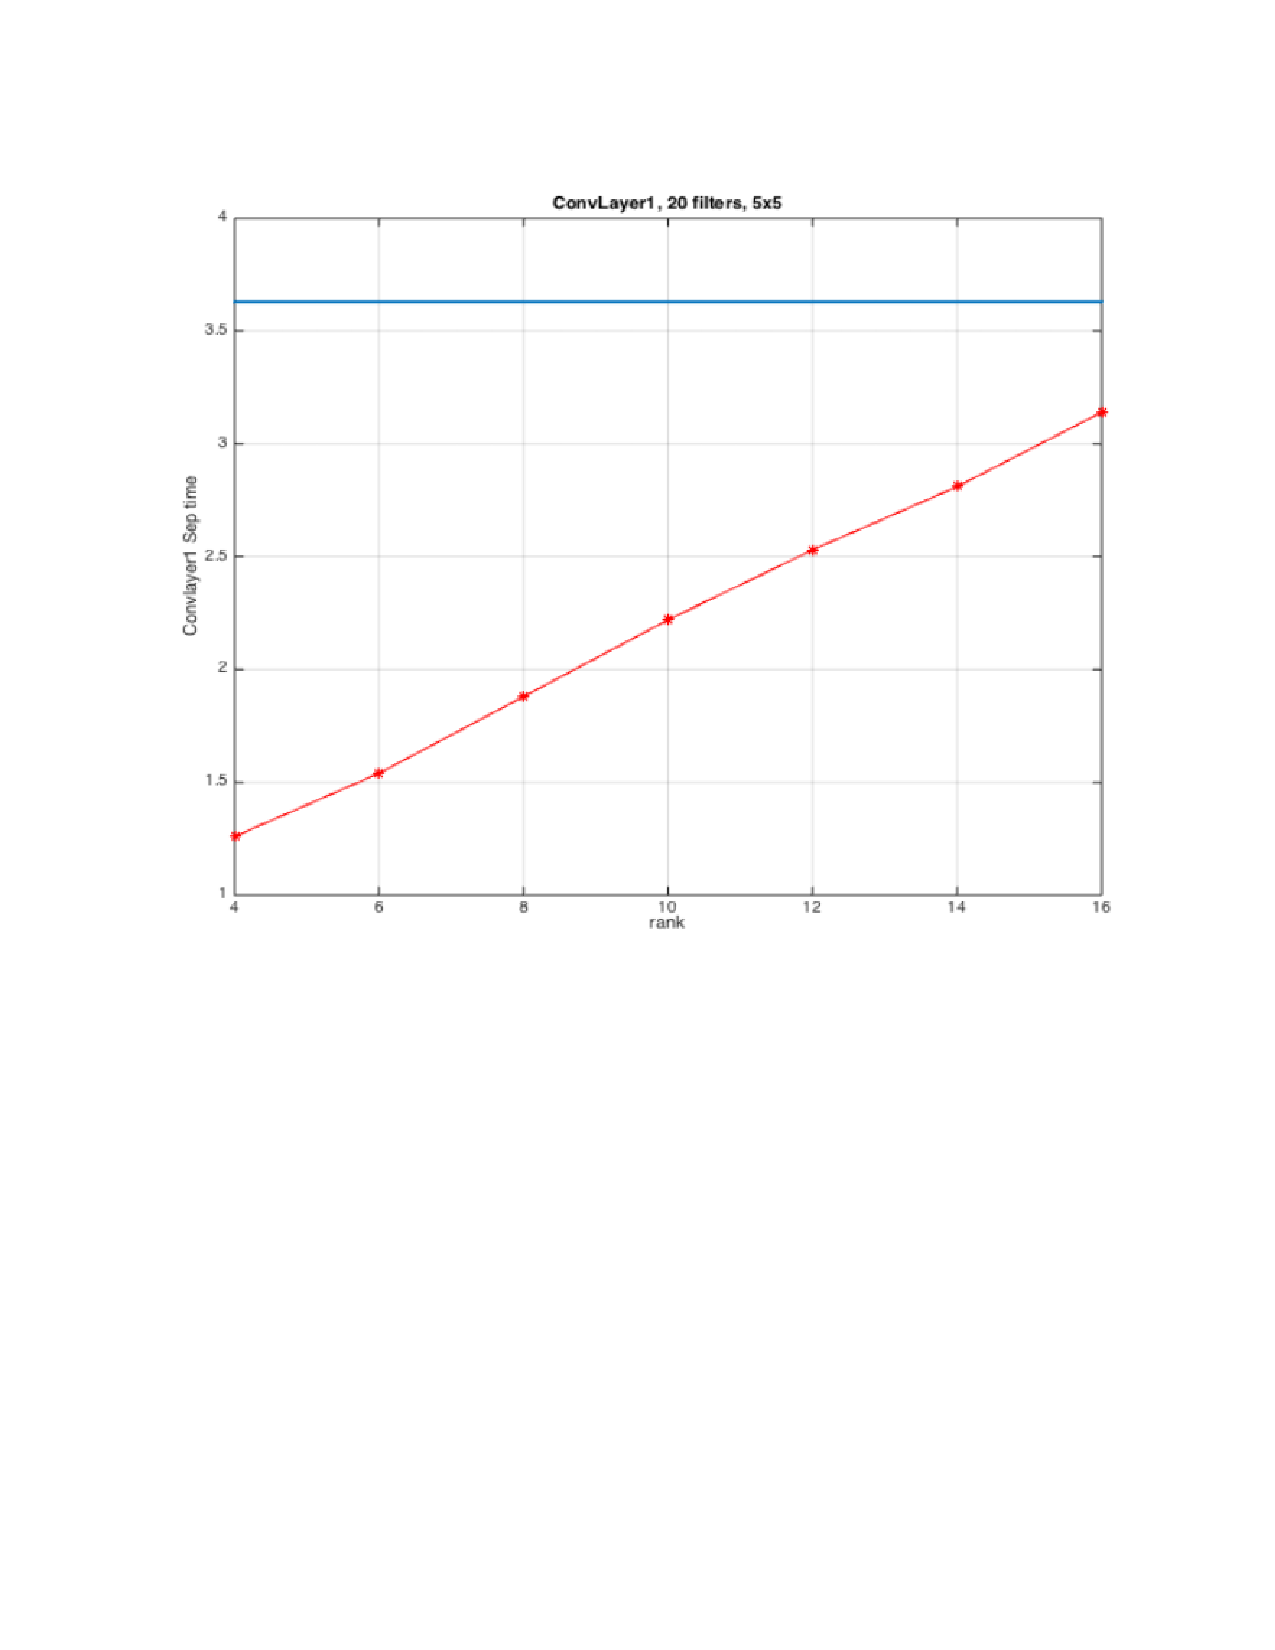
\includegraphics[width=\textwidth]{images/imagesCNN_page5.pdf}
    \caption{Convolutional layer 1}
  \end{subfigure}
  \begin{subfigure}[b]{0.40\textwidth}
    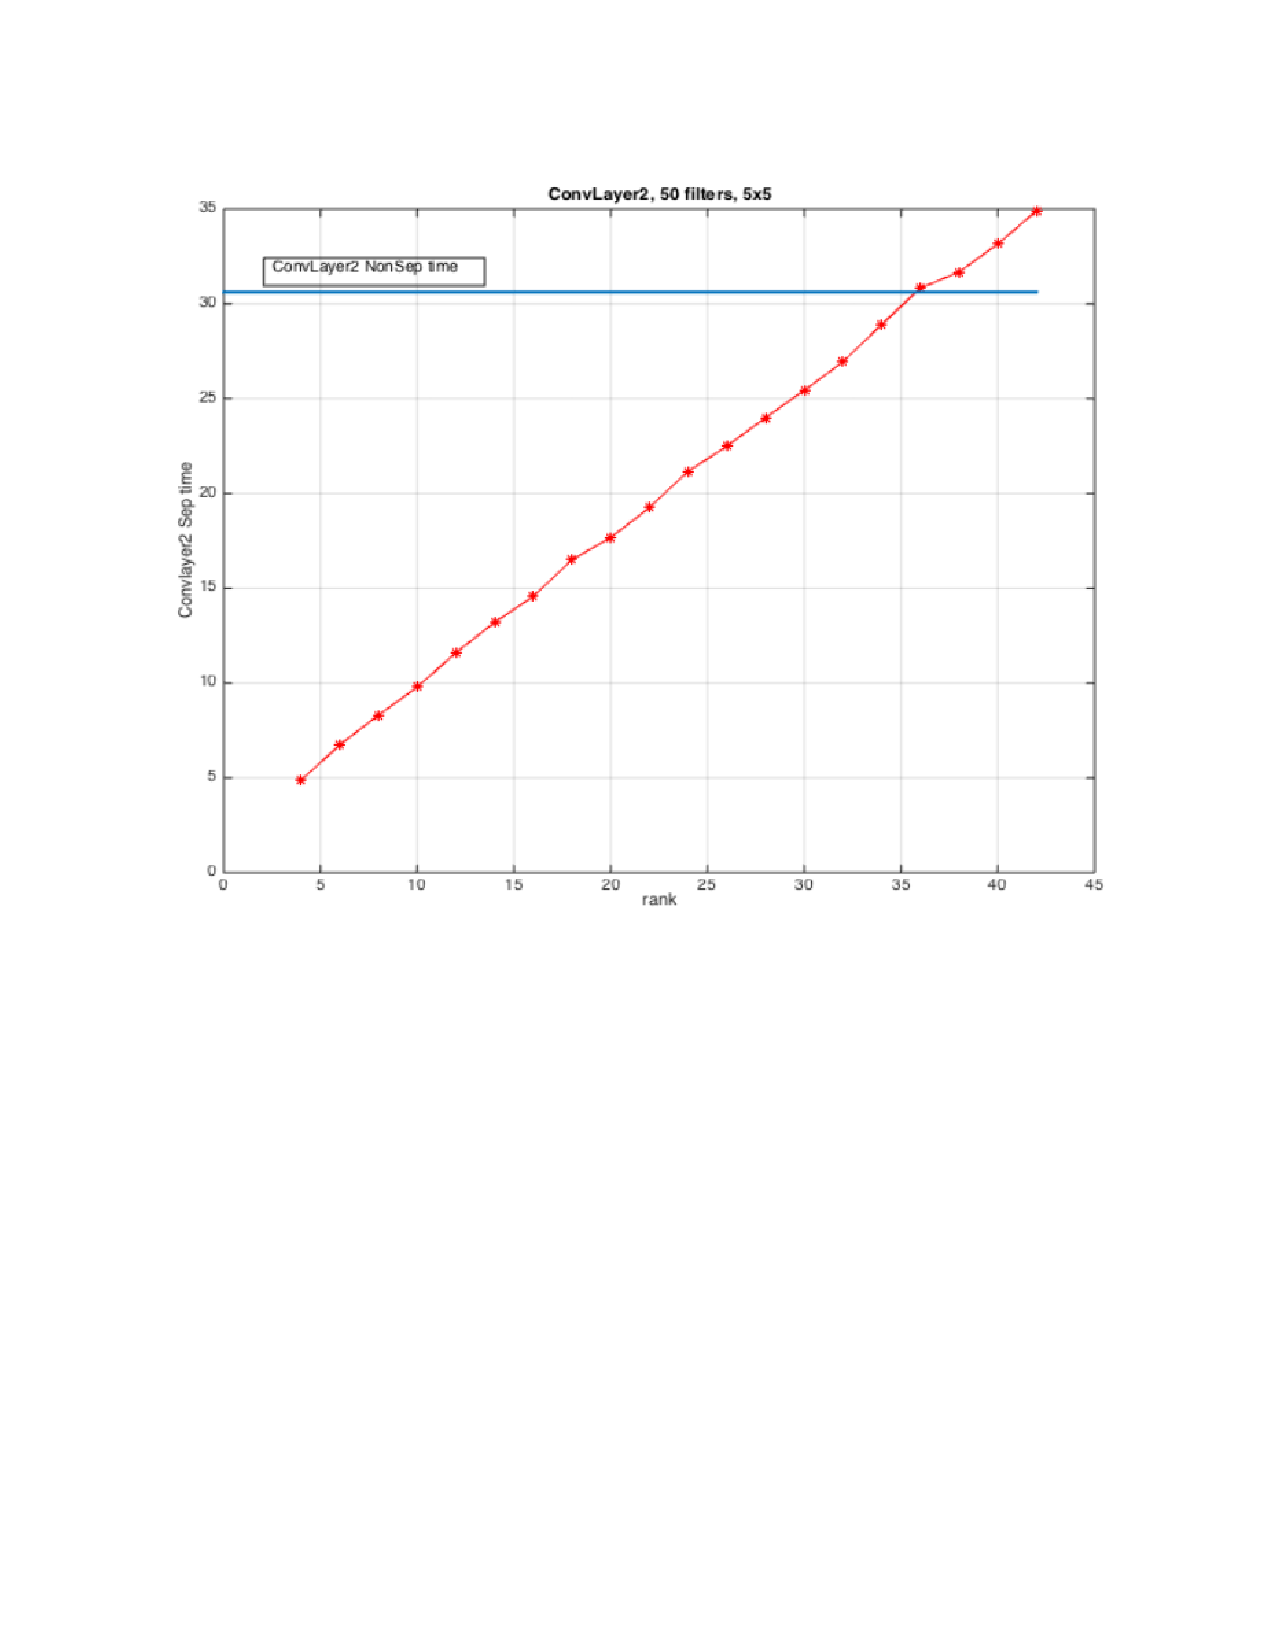
\includegraphics[width=\textwidth]{images/imagesCNN_page3.pdf}
    \caption{Convolutional layer 2}
  \end{subfigure}
  \caption{CNN Model 1 MNIST. Rank vs Time}
  \label{fig:cnn1time}
\end{figure}

The question that remains is to see how far we can afford to reduce the rank such that we do not lose much from the classification accuracy. Fig \ref{fig:cnn1error} a shows how the performance of the CNN drops with decreasing rank. With rank 16 the performance is the same, while for rank between 10 and 16 the error rate stays between 0.8 and 0.9 per cent, which is quite low. According to the application, even a rank of 8 or 6 is acceptable, since the drop is not more than 1 per cent.

\begin{figure}[h!]
  \centering
  \begin{subfigure}[b]{0.40\textwidth}
   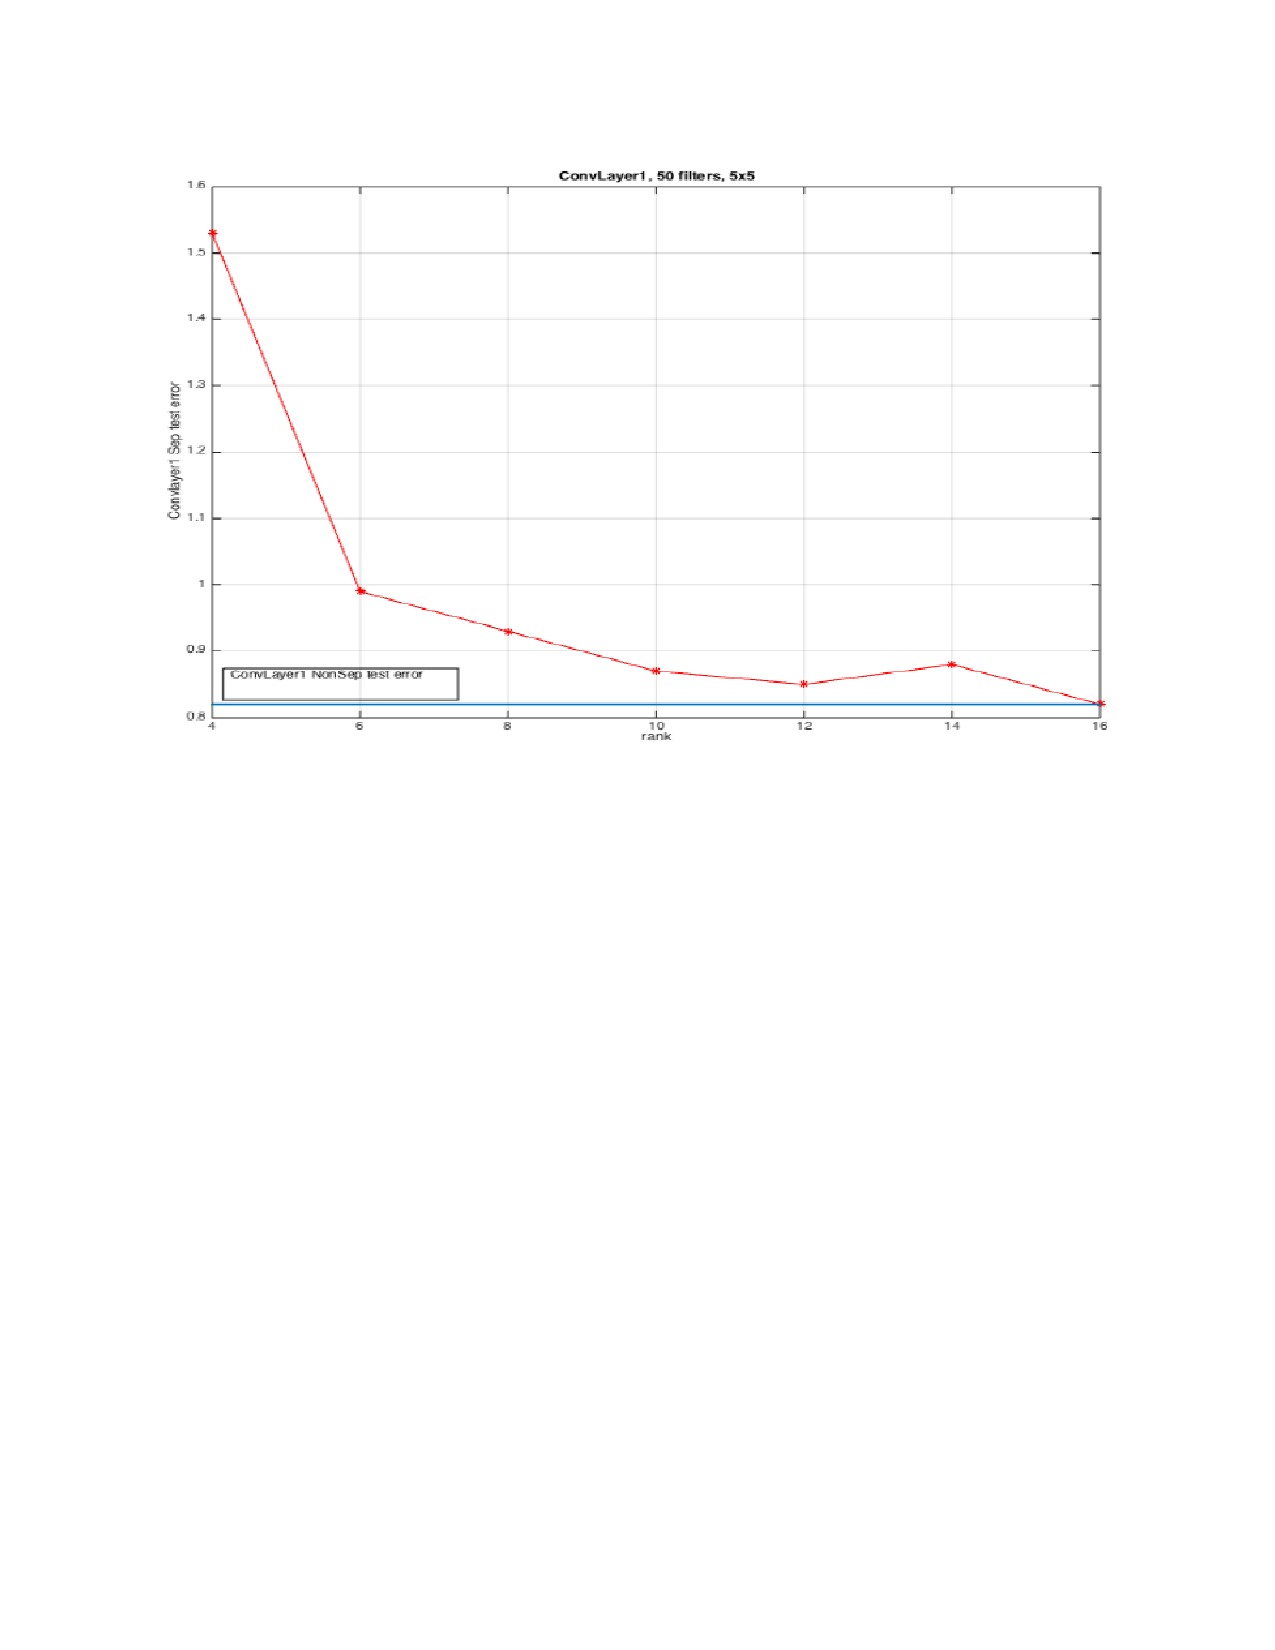
\includegraphics[width=\textwidth]{images/imagesCNN_page4.pdf}
    \caption{Convolutional layer 1}
  \end{subfigure}
  \begin{subfigure}[b]{0.40\textwidth}
    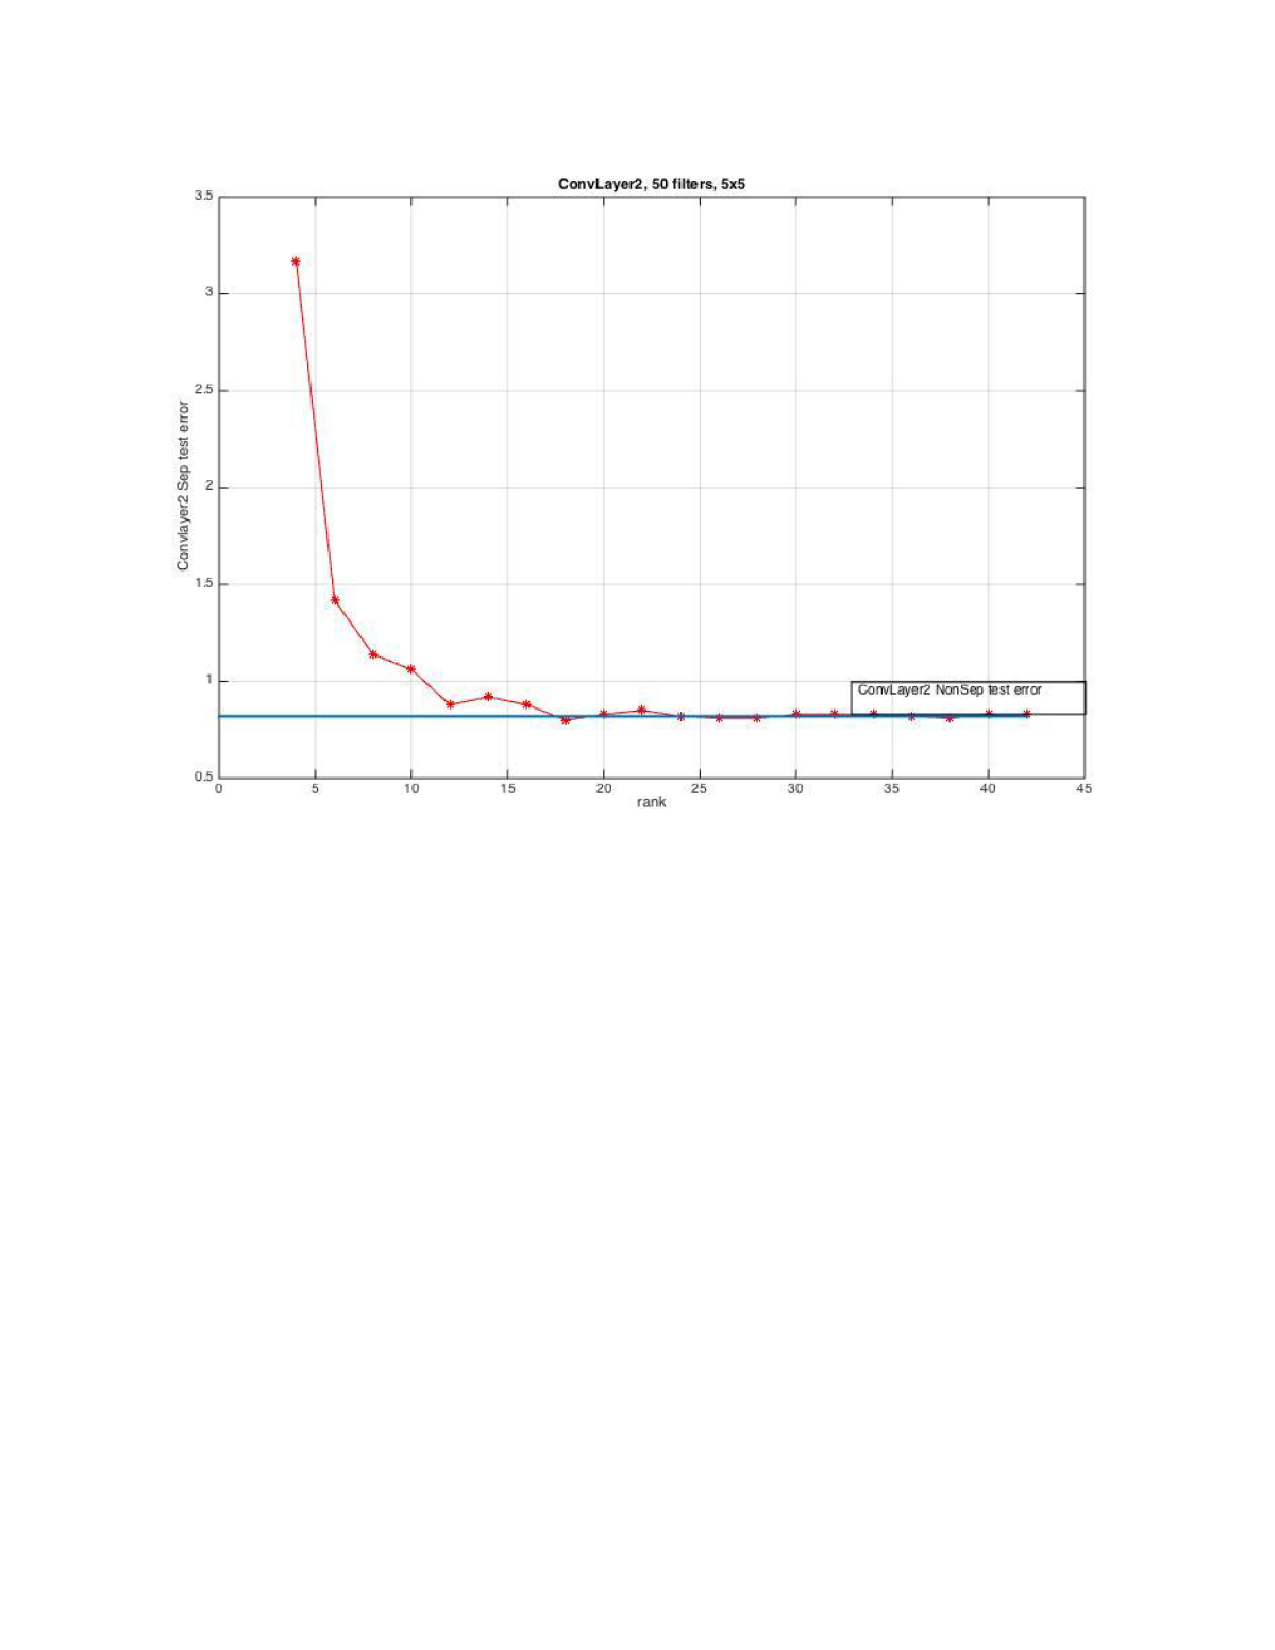
\includegraphics[width=\textwidth]{images/imagesCNN_page1.pdf}
    \caption{Convolutional layer 2}
  \end{subfigure}
  \caption{CNN Model 1 MNIST. Rank vs Error Rate}
  \label{fig:cnn1error}
\end{figure}

In the second experiment, we kept the first layer unchanged and approximated the second convolutional layer.
Similarly, according to Table \ref{table:rank}, we have a very tall tensor $R^{50\times 5 \times 5}$ with a typical rank of 25.
Fig\ref{fig:cnn1fitness}b shows how well is the approximation with varying rank from 4 to 42 in steps of 2 . As expected, the fit is almost perfect (99.9 fit) for rank higher than the theoretical one of 25.

From the complexity perspective, the separable CNN is faster if we use a rank $K << \frac{Jd_{1}d_{2}}{J +d_{1}+d_{2}} = 20.83$. In our case, for rank = 20 we obtained almost a 40$\%$ speedup. This is due as before to language specific implementation.
For rank 10, using separable filters is actually 3 times faster (theoretically 2 times faster).
If we keep the rank greater than 10, the recognition never drops more than 1 error rate.
For rank 12 the fit is 79 but the error rate is still almost unchanged which means we can easily use rank with relatively bad fit and still obtain good performance. Using separable filters of similar fit of 79  we obtained a slitghly lower performance. This might imply that it is more important to approximate well the first layer, which is the building block for the following layers.
\subsubsection{CNN Model 2}
In the following experiment, we keep the same number of filters per layers but increase the
kernel sizes to $9\times9$ Fig\ref{fig:CNN2}. We obtained a slightly lower performance for this set 1.3 error rate (compared with 0.82 for the previous model). In [cite here \textcolor{red}{find paper}]
they claim that using larger filters does not actually improve peformance of cnns since they struggle to learn bigger filters, but investigating this issue is not the goal of the report.
\begin{table}[h!]
\centering
\begin{tabular}{@{}rlll@{}}\toprule
Layer & Type & Maps and neurons& Kernel size \\ \midrule
0 & input & 1 map of 28x28 &\\
1& convolutional & 20 maps of 24x24 & 9x9\\
2 & max pooling & 20 maps of 12x12 &  \\
3 & convolutional & 50 maps of 8x8& 9x9 \\
4 & max pooling & 50 maps of 4x4&  \\ 
5 & fully conntected& 500 & \\
6 & fully conntected & 2 neurons & \\ \bottomrule
\end{tabular}
\caption{CNN Model 2  MNIST}
\label{fig:CNN2}
\end{table}
Here we only approximate convolutional layer 2 (rank from 4 to 18 with corresponding fit between 45 and 90). The theoretical rank is less than 49 and we obtain speedup if the rank $K << 59.5$
The results can be seen in Fig\ref{fig:cnn2error}. We notice that up to rank 8 the error of the Separable CNN is reasonable and does not drop more than 1.6 (1.3 is the reference error of the non separable CNN). The speedup for conv L2 drops from 15ms to 12 ms for rank 18 , which is actually much smaller than we expected for using larger filters.
\begin{figure}[h!]
  \centering
  \begin{subfigure}[b]{0.40\textwidth}
   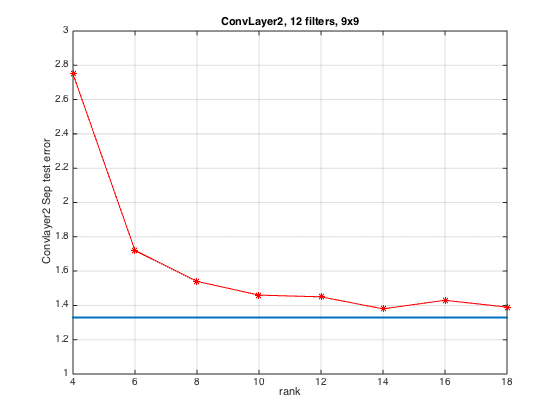
\includegraphics[width=\textwidth]{presentation_plots/convL2_error.png}
    \caption{Conv L2 - Rank vs Error}
  \end{subfigure}
  \begin{subfigure}[b]{0.40\textwidth}
    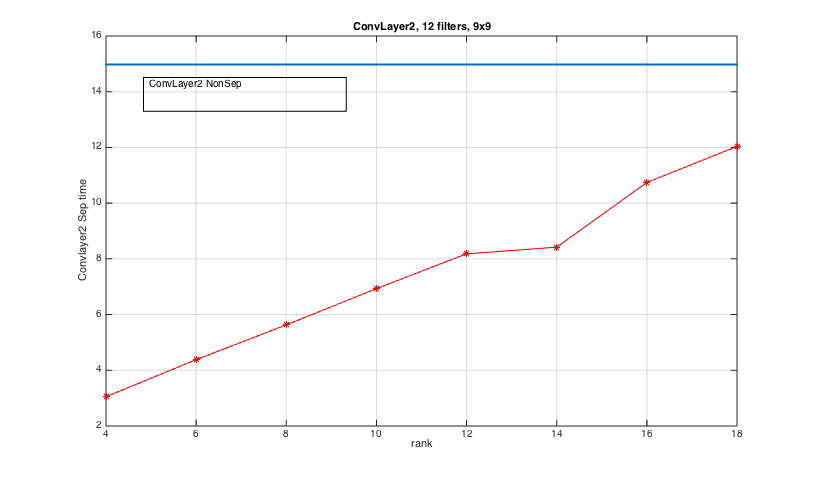
\includegraphics[width=\textwidth]{presentation_plots/convL2_time.png}
    \caption{Conv L2 - Rank vs Time}
  \end{subfigure}
  \caption{CNN Model 2 MNIST.}
  \label{fig:cnn2error}
\end{figure}

\subsection{Mitocondria Striatum}
For the Mitocondria Striatum set, CNN are employed to solve a segmentation problem. Every pixel is classified as being part of the mitocondria or not. A patch of 51x51 surrounding the pixel is extracted from the image and fed as input to a CNN which acts as a binary classifier. For determining the parameters of the CNN we used a set of
100.000 samples for training and 20.000 for validation (containing half positive and half negative samples). After determining the best setup, the network was trained on a larger set of 1 milion samples for training and 200.000 for validation.

The final test data represented a 3D image volume consisting of 318 slices of size 400x661. Thus, one frame contains 264.400 datasamples that are fed as test input for the CNN, while all frames contain 97 million datasamples.

The best setup obtained using the small training and validation set was the one presented in Fig\ref{fig:CNN3} NonSep. This gave us a VOC error on the first frame of 77.2. We then trained this net on the big set and obtained an error of 74. We notice that this is not comparable with state of the art methods which achieve results higher than 79 VOC or that use 3D information. The goal of this
is to see if we can obtain a speedup by using separable filters.
\begin{table}
\centering
\begin{tabular}{@{}rlll@{}}\toprule
Layer & Type & Maps and neurons& Kernel size \\ \midrule
0 & input & 1 map of 51x51 &\\
1& convolutional & 10 maps of 46x46 & 6x6\\
2 & max pooling & 10 maps of 23x23 &  \\
3 & convolutional & 20 maps of 18x18& 6x6 \\
4 & max pooling & 20 maps of 9x9& \\ 
3 & convolutional & 50 maps of 4x4& 6x6 \\
4 & max pooling & 50 maps of 2x2& \\ 
5 & fully conntected& 100 & \\
6 & fully conntected & 2 neurons & \\ \bottomrule
\end{tabular}
\caption{CNN for Mitocondria set}
\label{fig:CNN3}
\end{table}
Example of the weights learned in the first convolutional layer are shown in Fig[ref] and of output on one frame produced by the CNN. 
\begin{table}
\centering
\begin{tabular}{@{}rllll@{}}\toprule
 &&Conv L1& Conv L2 & Conv L3\\ \midrule
NonSep &Kernel Size & 10 maps 6x6& 20 maps 6x6 & 50 maps 6x6\\
&Speedup rank& $\leq$16.36 & $\leq$22.5 & $\leq$29.03\\
&Theoretical rank & 16.4 & $\leq$36 & 36 \\ 
&time & 8.1 & 26.8 & 18.4 \\ \midrule
Separable& rank & - & 20 & 36 \\ 
& time& - & 20.1 & 17.6\\ \midrule
\end{tabular}
\caption{CNN for Mitocondria set}
\label{fig:CNN3}
\end{table}
\begin{figure}[h!]
  \centering
  \begin{subfigure}[b]{0.40\textwidth}
   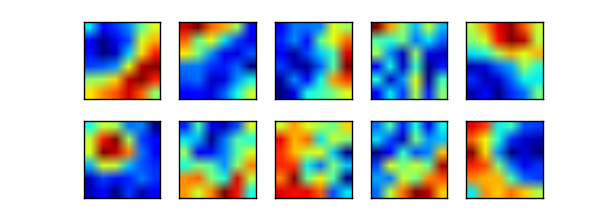
\includegraphics[width=\textwidth]{images/filters.png}
    \caption{Weights learned in the 1st layer}
  \end{subfigure}
  \begin{subfigure}[b]{0.40\textwidth}
    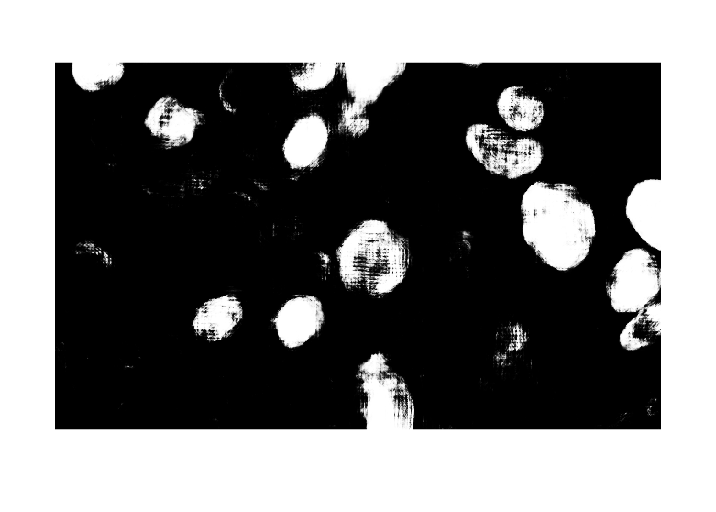
\includegraphics[width=\textwidth]{images/frame1.png}
    \caption{CNN output frame, not thresholded}
  \end{subfigure}
    \begin{subfigure}[b]{0.40\textwidth}
   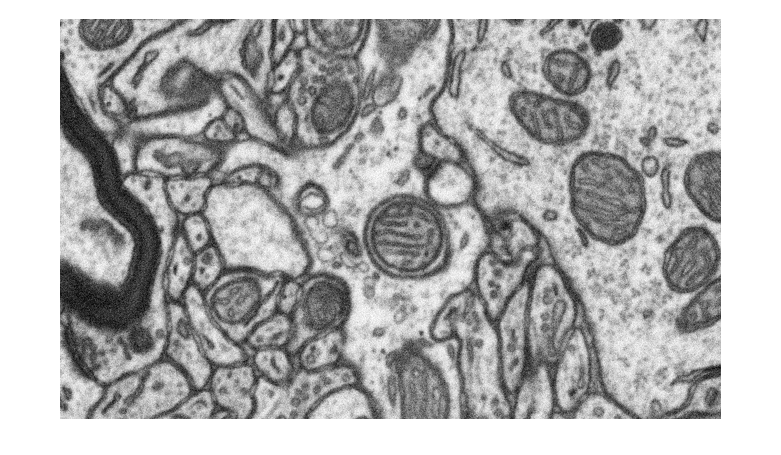
\includegraphics[width=\textwidth]{images/GT_truth.png}
    \caption{CNN input frame}
  \end{subfigure}
  \begin{subfigure}[b]{0.40\textwidth}
    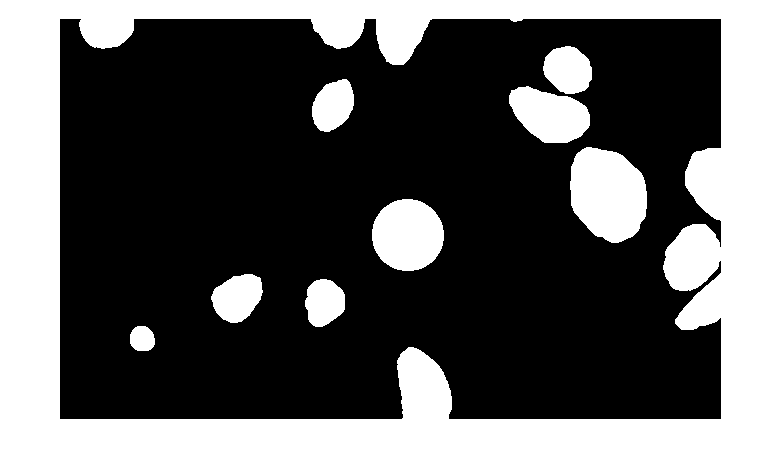
\includegraphics[width=\textwidth]{images/GTframe1.png}
    \caption{Groundtruth frame}
  \end{subfigure}
  \caption{Input and output example of CNN for mitocondria dataset. Fig a) shows that the filters are mostly edge and circle detectors which constitute basic building blocks for the interior of the mitocondria.
  Comparing b), c) and d) we notice the 'noisy' nature of the CNN output for pixel classification. Preprocessing the final output b) using a median filter would likely improve the results.}
  \label{fig:mitocondria}
\end{figure}
We keep conv L1 fixed and approximate conv L2 and L3 with rank 20 and 36 respectively. For the 3rd layer no significant change in performance is observed, while for layer 2 we notice a small speedup from roughly 26 to 20 ms. Since the fit of the two layers was very good (99.9) there was no drop in classification performance.

Fig \ref{fig:mitocondria} shows an example of the CNN input and output and the type of filters that it learns. 


\subsection{Pre trained ImageNet CNN}
We investigated if we could theoretically speedup CNNs of large networks, like the ones used in ImageNet challenge. The network below is the reference net from Alex Kristevski paper (without the split to be run on two GPUs). The net was trained by [cite].

We  

\begin{figure}[h]
  \centering
  \begin{subfigure}[b]{0.40\textwidth}
   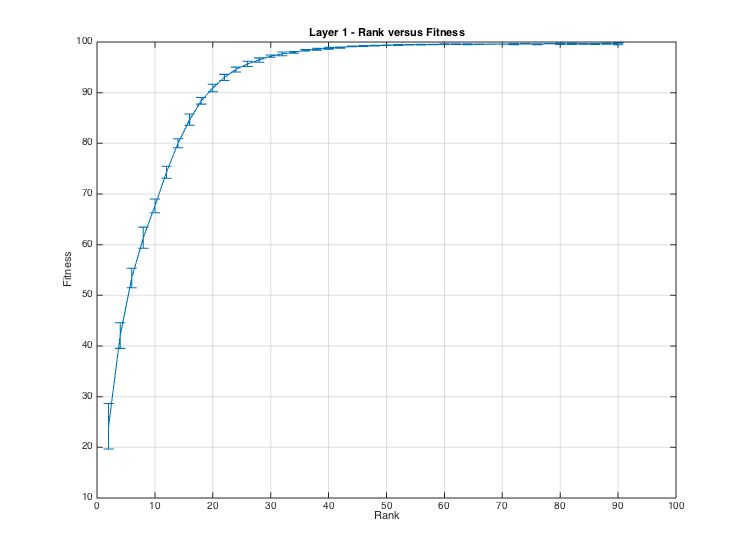
\includegraphics[width=\textwidth]{images/Layer1ImageNet.png}
    \caption{}
  \end{subfigure}
  \begin{subfigure}[b]{0.40\textwidth}
    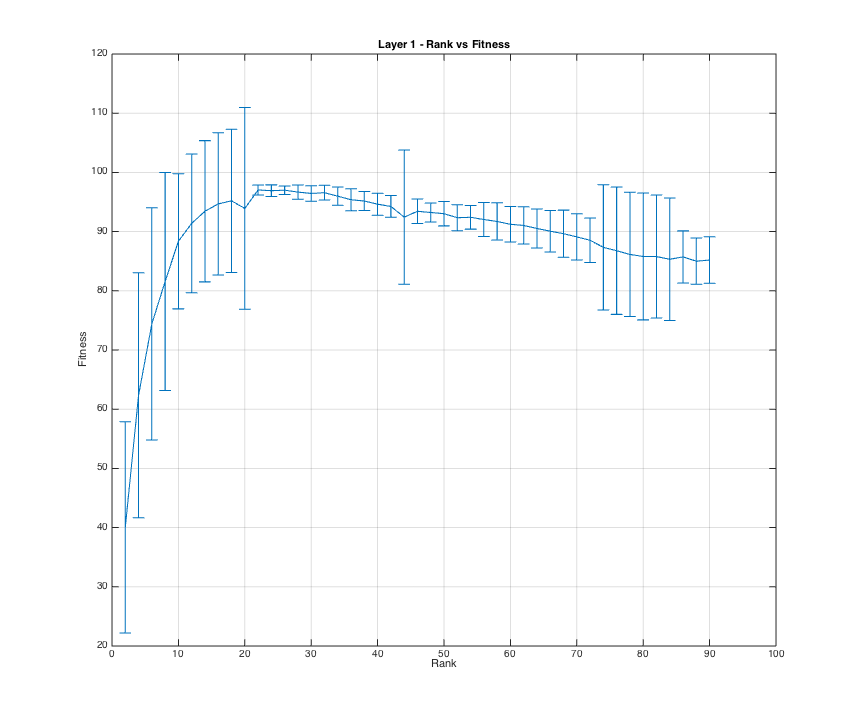
\includegraphics[width=\textwidth]{images/Layer2ImageNet.png}
    \caption{}
  \end{subfigure}
  \caption{ImageNet Layers}
  \label{fig:user_stribution}
\end{figure}

\begin{figure}[h]
  \centering
  \begin{subfigure}[b]{0.40\textwidth}
   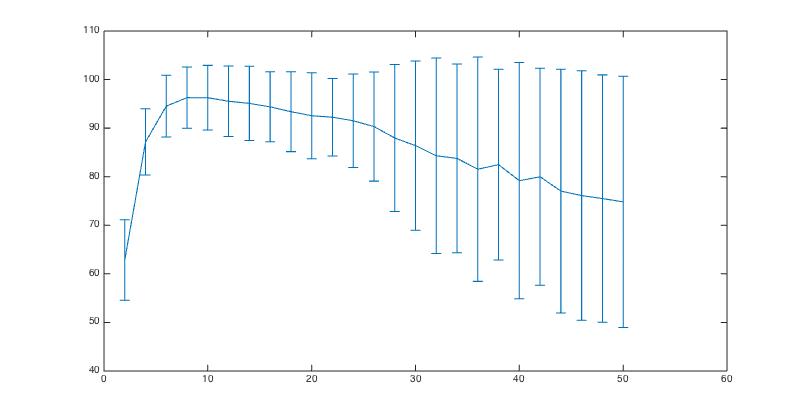
\includegraphics[width=\textwidth]{images/Layer3ImageNet.png}
    \caption{}
  \end{subfigure}
  \begin{subfigure}[b]{0.40\textwidth}
    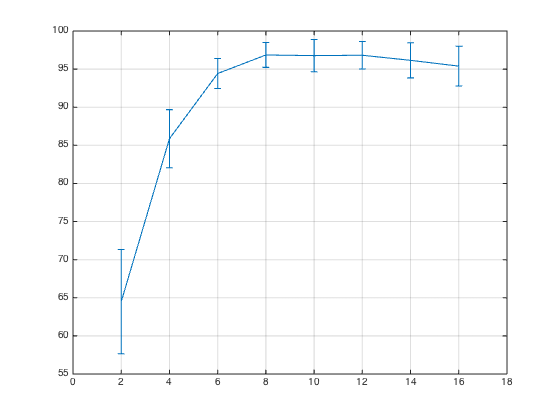
\includegraphics[width=\textwidth]{images/Layer4ImageNet.png}
    \caption{}
  \end{subfigure}
  \caption{ImageNet Layers}
  \label{fig:user_artiststribution}
\end{figure}

\section{Conclusions}
Theoretical bounds of the separabe filters choice are proven.


\section*{Acknowledgments}
I would like to thank Simon Arosi that helped me a lot during this project giving me constant feedback.

\bibliography{citations}
\bibliographystyle{plain}

\end{document}

